%!TEX TS-program = Arara
% arara: pdflatex: { draft : yes }
% arara: biber
% arara: makeindex
% arara: pdflatex
\documentclass[ngerman,11pt,parskip=half,liststotoc,bibtotoc,oneside]{scrbook} %

\usepackage[top=5mm,left=5mm,bottom=5mm,right=5mm]{geometry}

%\usepackage[grid, gridunit=mm, texcoord, gridcolor=blue, subgridcolor=gray!50]{eso-pic}

\usepackage{booktabs}
\usepackage{index}
\makeindex

\author{Uwe Ziegenhagen}
\title{Meine Dissertation CO\textsubscript{2} CO2}
\date{Köln, den \today}

\usepackage[headsepline=0.5pt,footsepline=0.5pt]{scrlayer-scrpage}
\KOMAoptions{headwidth=1.1\textwidth,footwidth=1.1\textwidth}

\pagestyle{scrheadings}
\clearscrheadings 

\clearscrheadings 
\ohead[]{\headmark}
\ofoot{\pagemark}
\ihead{}
\ifoot{}
\chead{}
\cfoot[\pagemark]{}


\usepackage{booktabs}
\usepackage{babel}
\usepackage{graphicx}
\usepackage{csquotes}
\usepackage{paralist}
\usepackage{xcolor}
\usepackage{blindtext}
\usepackage{chemformula}
\usepackage{siunitx}

\usepackage[style=authortitle-icomp,backref,backend=biber]{biblatex}

\addbibresource{Literatur.bib}

% Schmutzige Hacks
%\setlength{\parindent}{0pt}
%\setlength{\parskip}{6pt}

\usepackage{hyperref}
\hypersetup{
    bookmarks=true,                     % show bookmarks bar
    unicode=false,                      % non - Latin characters in Acrobat’s bookmarks
    pdftoolbar=true,                        % show Acrobat’s toolbar
    pdfmenubar=true,                        % show Acrobat’s menu
    pdffitwindow=false,                 % window fit to page when opened
    pdfstartview={FitH},                    % fits the width of the page to the window
    pdftitle={My title},                        % title
    pdfauthor={Author},                 % author
    pdfsubject={Subject},                   % subject of the document
    pdfcreator={Creator},                   % creator of the document
    pdfproducer={Producer},             % producer of the document
    pdfkeywords={keyword1, key2, key3},   % list of keywords
    pdfnewwindow=true,                  % links in new window
    colorlinks=true,                        % false: boxed links; true: colored links
    linkcolor=blue,                          % color of internal links
    filecolor=blue,                     % color of file links
    citecolor=blue,                     % color of file links
    urlcolor=blue                        % color of external links
}
 

\makeatletter
%https://tex.stackexchange.com/questions/239490/how-can-i-print-a-length-in-centimeters
\def\convertto#1#2{\strip@pt\dimexpr #2*65536/\number\dimexpr 1#1}
\makeatother

\begin{document}
\maketitle

\frontmatter
\tableofcontents

\listoffigures

\listoftables

\clearpage
\addcontentsline{toc}{chapter}{Abkürzungsverzeichnis}
\chapter*{Abkürzungsverzeichnis}

\begin{tabular}{lp{0.75\textwidth}} \toprule
Kürzel & Erläuterung \\ \midrule
$\pi$ & Kreiszahl \\ \bottomrule
\end{tabular}

\mainmatter

\index{Physiker!Einstein} \index{Physiker!Meitner}

\chapter{Test}

Textbreite \convertto{cm}{\the\textwidth} cm, Texthöhe \convertto{cm}{\the\textheight} cm



%!TEX TS-program = Arara
%!TeX root = Hauptdokument.tex
\chapter{Einführung}\label{cha:einführung}
\section{Literatur}

\cite{knuth:1984} 

\blindtext[1] Hallo, ich mag die Arbeit mit \LaTeX.

\si{\micro\meter}

\blindtext[1]

\blindtext[1]

\blindtext[1]

\blindtext[2]


\section{Historischer Abriss}

\blindtext[5]


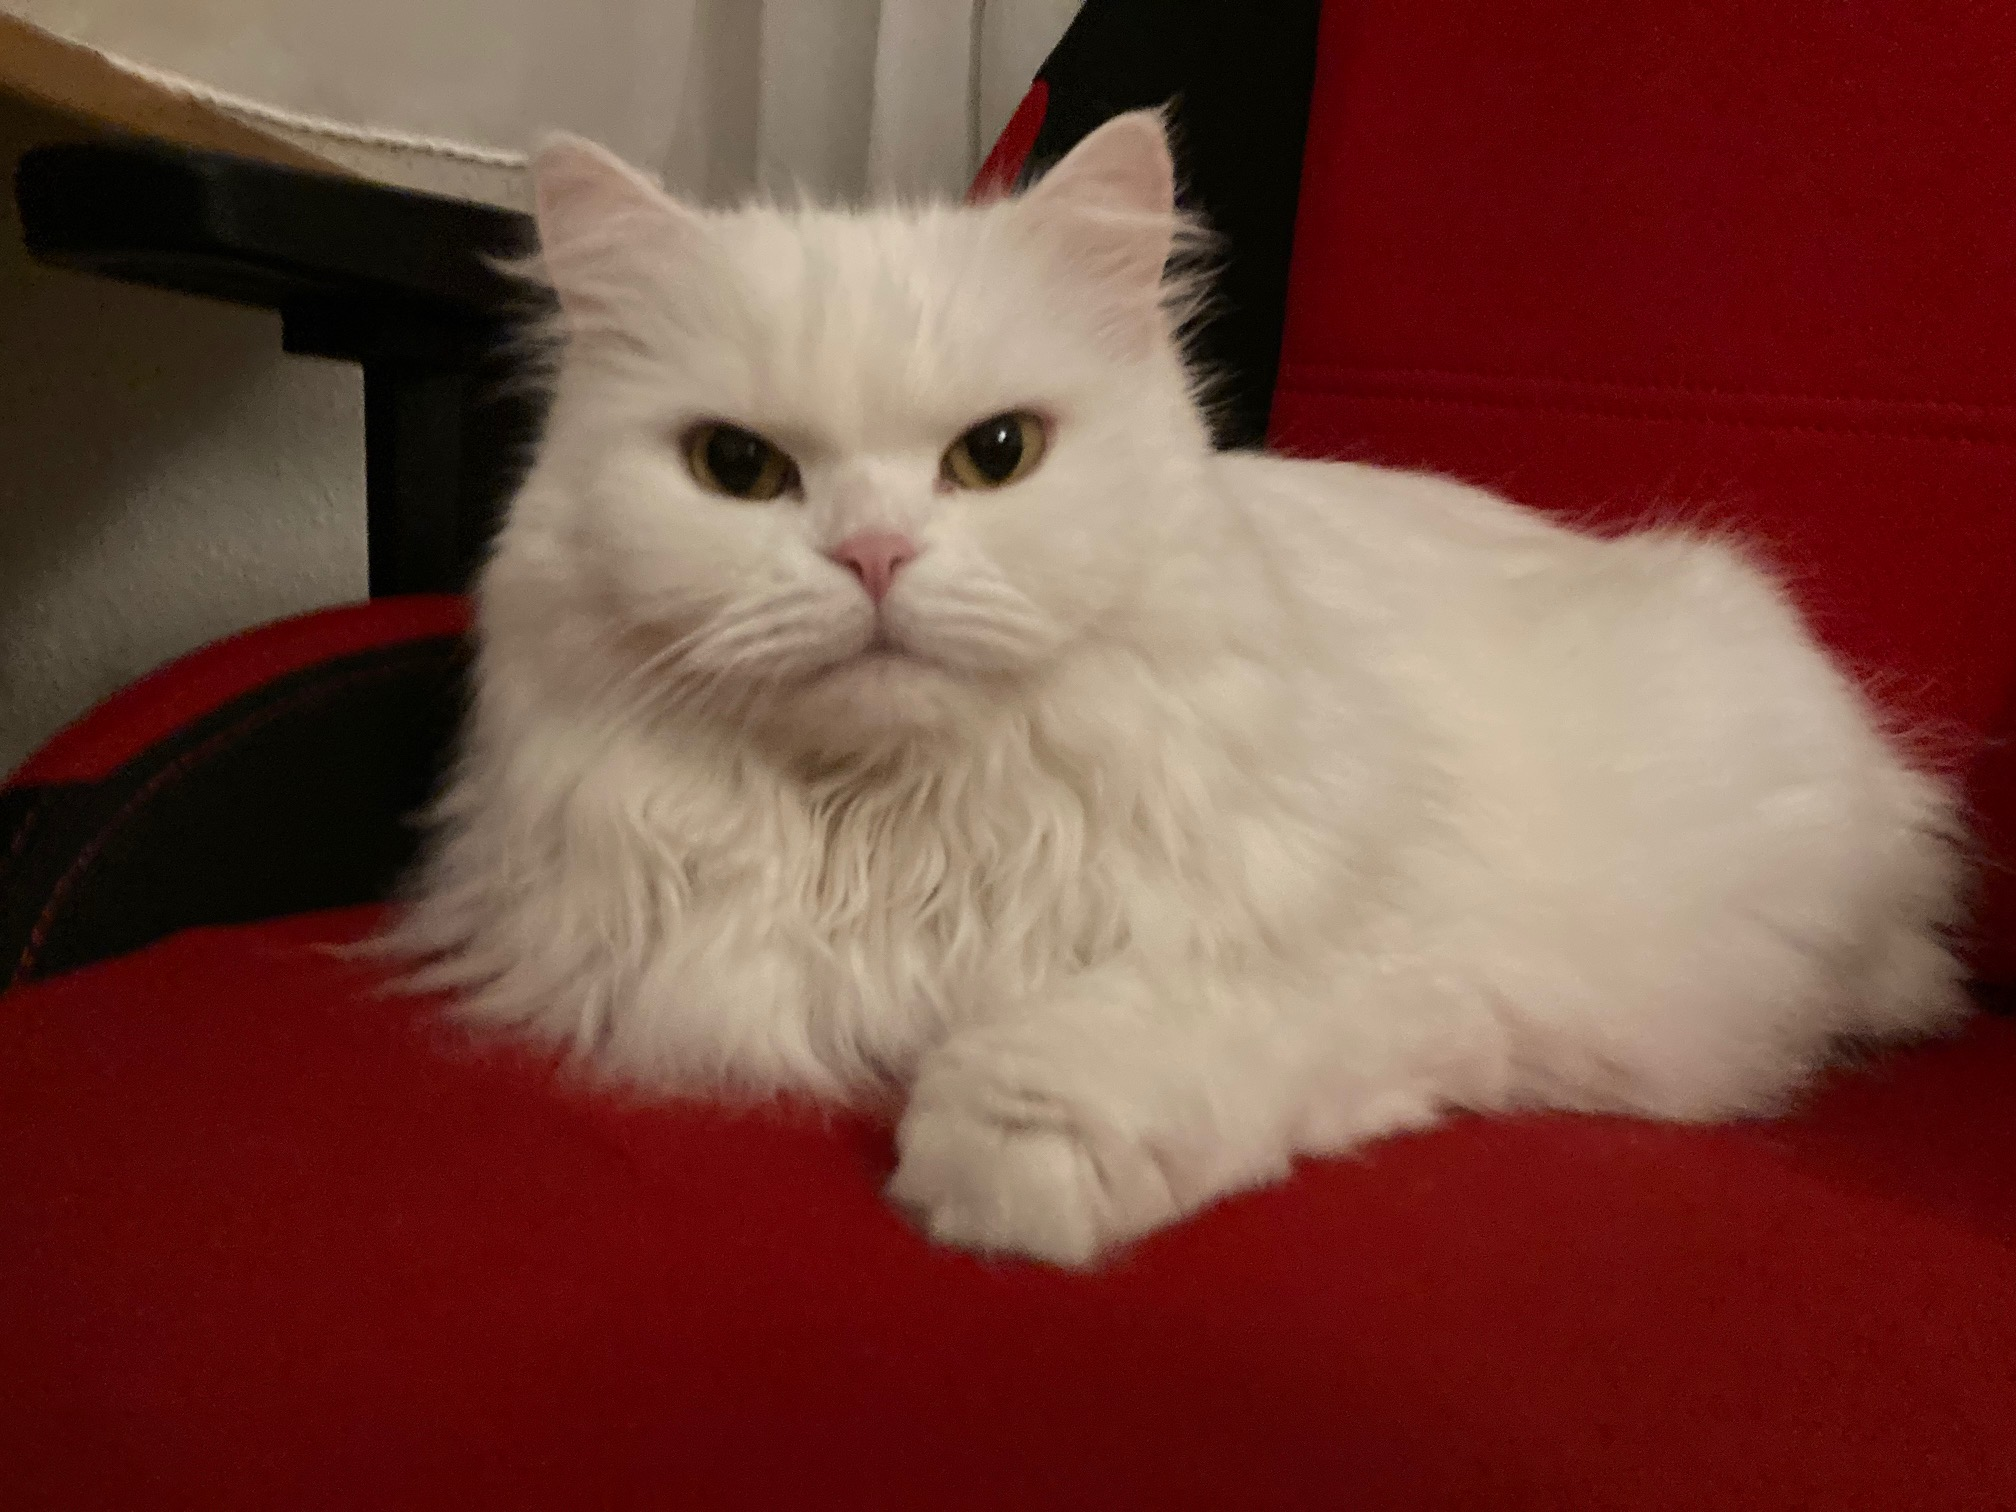
\includegraphics[width=\textwidth]{Bilder/Katze2}

%!TEX TS-program = Arara
%!TeX root = Hauptdokument.tex
\chapter{Hauptteil}\label{cha:hauptteil}
\section{Stand der Forschung}

\cite{kohm:2018} \citeyear{kohm:2018}

\blindtext[1] Hallo, ich mag die Arbeit mit \LaTeX.

\si{\micro\meter}

\blindtext[1]

\blindtext[1]

\blindtext[1]

\blindtext[2]


\section{Herausforderungen beim Einsatz von kryptonitischen Plasma-Strahlengeneratoren im ostasiatischen Raum unter Gesichtspunkten der Ethik}

\blindtext[5]


%!TEX TS-program = Arara
%!TeX root = Hauptdokument.tex
\chapter{Fazit}\label{cha:fazit}
\section{Zusammenfassung}

\cite{kohm:2018} \citeyear{kohm:2018}

\blindtext[1] Hallo, ich mag die Arbeit mit \LaTeX.

\si{\micro\meter}

\blindtext[1]

\blindtext[1]

\blindtext[1]

\blindtext[2]


\section{Ausblick}

\blindtext[5]



\backmatter
\chapter{Anhang}

\printindex

% böse
%\nocite{*}
\printbibliography

\end{document}